\documentclass{beamer}

% Style
\usepackage{xcolor}

\usetheme{Madrid}
\usepackage{dirtree}
% Color
\definecolor{flatblue}{RGB}{106, 137, 204}
\usecolortheme[named=flatblue]{structure}
% Font
\usepackage{emoji}
\usepackage{fontspec}
\usepackage{csquotes}
\setsansfont{EB Garamond}
% Code
\usepackage{listings}
\usepackage{graphicx}
\usepackage{hyperref}
\hypersetup{
    colorlinks=true,
    linkcolor=flatblue,
    filecolor=flatblue,
    urlcolor=flatblue,
    citecolor=flatblue
}
\definecolor{flatgreen}{RGB}{0, 98, 102}
\definecolor{flatgreyish}{RGB}{209, 216, 224}
\lstset{
    basicstyle=\ttfamily\scriptsize,
    backgroundcolor=\color{flatgreyish},
    keywordstyle=\color{flatgreen},        % Keywords font ('*' = uppercase)
    commentstyle=\color{flatblue},         % Step between two line-numbers
    columns=fullflexible,
    breaklines=true
}

% Highlight
\usepackage[most]{tcolorbox}
\usepackage{cleveref}
\crefformat{footnote}{#2\footnotemark[#1]#3}
\usepackage{amsmath}
\definecolor{flatorange}{RGB}{255, 165, 2}
\definecolor{flatred}{RGB}{255, 71, 87}
\tcbset{textmarker/.style={%
skin=enhancedmiddle jigsaw,breakable,parbox=false,
boxrule=0mm,leftrule=2mm,rightrule=0mm,boxsep=0mm,arc=0mm,outer arc=0mm,
left=1mm,right=1mm,top=1mm,bottom=1mm,toptitle=1mm,bottomtitle=1mm}}
\newtcolorbox{dangercolorbox}{textmarker,colback=flatorange,colframe=flatred}

% Title
\title{Mise en production et déploiement - MS2D / ERIS}
\author{Christophe Brun}
\institute{Campus Saint-Michel IT}
\date{17 avril 2024}
\beamertemplatenavigationsymbolsempty

% Graphix with arrows in between
\newcommand*{\vcenterimage}[1]{\vcenter{\hbox{\includegraphics[width=5cm]{#1}}}}
\newcommand*{\vcenterarrow}{\vcenter{\hbox{$\Longrightarrow$}}}

\titlegraphic{
    \bigbreak
    
\includegraphics[width=2cm]{image/logo-papit.png}
    
\includegraphics[width=2cm]{image/logo-campus-saint-michel-it.png}
}
\begin{document}

    \begin{frame}
        \transdissolve
        \titlepage
    \end{frame}

    \begin{frame}{Table des matières}
        \tableofcontents
    \end{frame}


    \section{Programme du module}
    \begin{frame}
        \frametitle{Mise en production et déploiement}
        \framesubtitle{Compétence acquise aucours des 5 jours du module}
        \transdissolve
        Compétences~:
        \begin{itemize}
            \item \textquote{Préparer l’environnement et déployer le progiciel ou la solution.}
        \end{itemize}
        \bigbreak
        \centering
        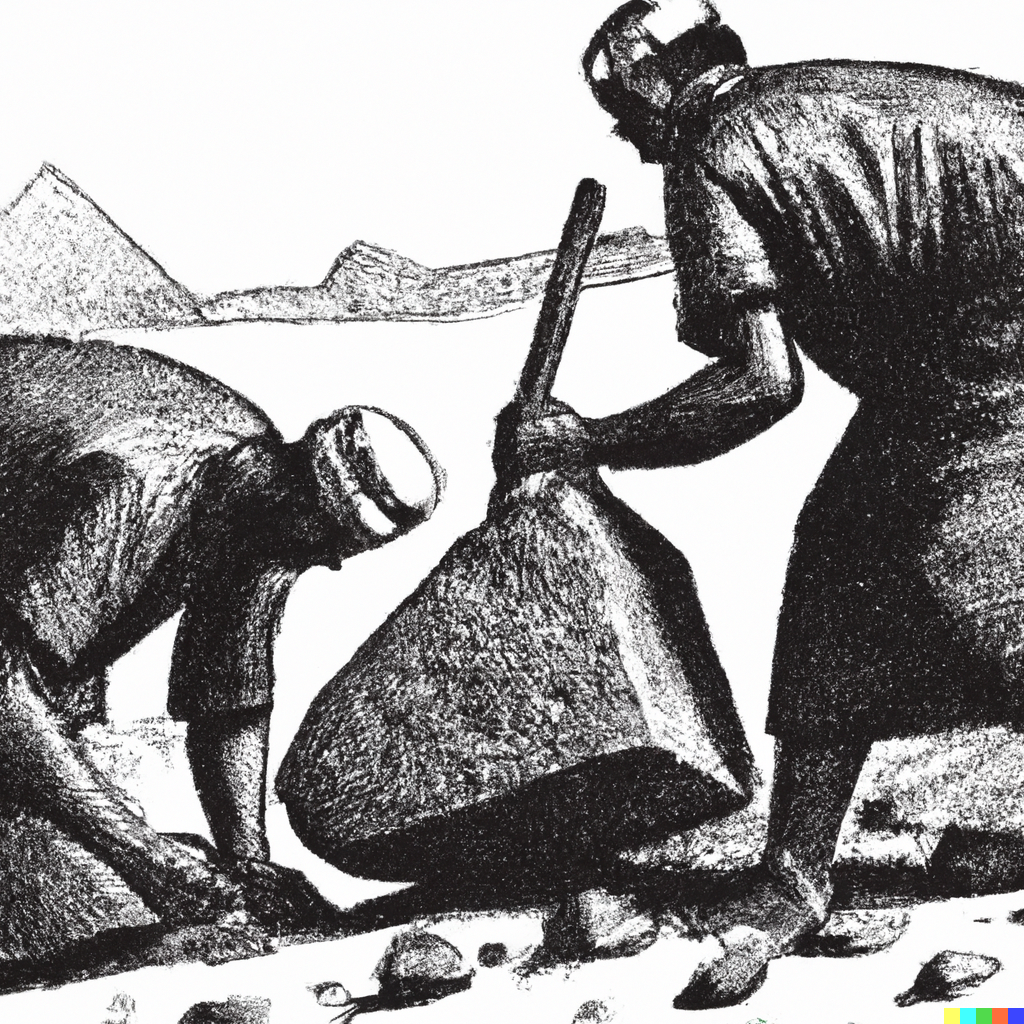
\includegraphics[width=5cm]{image/engraving-of-egyptian-workers-pulling-stones.png}
    \end{frame}

    \begin{frame}
        \frametitle{Mise en Production et déploiement}
        \framesubtitle{Le programme officiel des 5 jours du module}
        \transdissolve
        \begin{enumerate}
            \item Mise en exploitation des ressources matérielles et logicielles
            \begin{itemize}
                \fontsize{8pt}{8pt}\selectfont
                \item Vérification des configurations
                \item Déploiement des applications
                \item Automatisation des procédures de déploiement
                \item Élaborer les bilans de l’exploitation
                \item Prévoir les évolutions de l’infrastructure
            \end{itemize}
            \item Indicateurs et mesure de performances – Systèmes / Réseau et web
            \begin{itemize}
                \fontsize{8pt}{8pt}\selectfont
                \item Centralisation des journaux et exploitation des logs avec syslogd
                \item Analyse du trafic réseau avec MRTG
                \item Analyse des journaux de type d'Apache Web Server avec Analog
                \item Consolidation d'indicateur de qualité avec rrdtool
                \item Création de page HTML de type tableau de bord avec rrdtool – Tableau de bord
                \item Gestion d’incidents et actions correctives
            \end{itemize}
        \end{enumerate}
    \end{frame}

    \begin{frame}
        \transdissolve
        \frametitle{Evaluation}
        \begin{itemize}
            \item Bons points tout au long du module.
            \item 40 \% x 2 sur chaque séance de travaux pratiques.
            \item 20 \% sur une évaluation écrite finale
        \end{itemize}
    \end{frame}

    \begin{frame}
        \transdissolve
        \frametitle{Intervenant sur le module Architecture d'Aplication}
        \framesubtitle{Christophe Brun, conseil en développement informatique}

        \begin{columns}
            \column{0.7\textwidth}
            \begin{itemize}
                \item 1\textsuperscript{ere} année d'intervenant à Saint-Michel \emoji{star-struck}.

                \item 7 ans de conseil en développement au sein d'SSII.

                \item 7 ans de conseil en développement à mon compte \href{https://papit.fr}{PapIT}.

                \item Passionné~!
                \bigbreak
                \begin{columns}
                    \column{0.5\textwidth}
                    \centering
                    
\includegraphics[width=3cm]{image/logo-uppa.png}
                    \column{0.5\textwidth}
                    \centering
                    
\includegraphics[width=3cm]{image/logo-universite-bordeaux.png}
                \end{columns}
            \end{itemize}
            \column{0.3\textwidth}
            \centering
            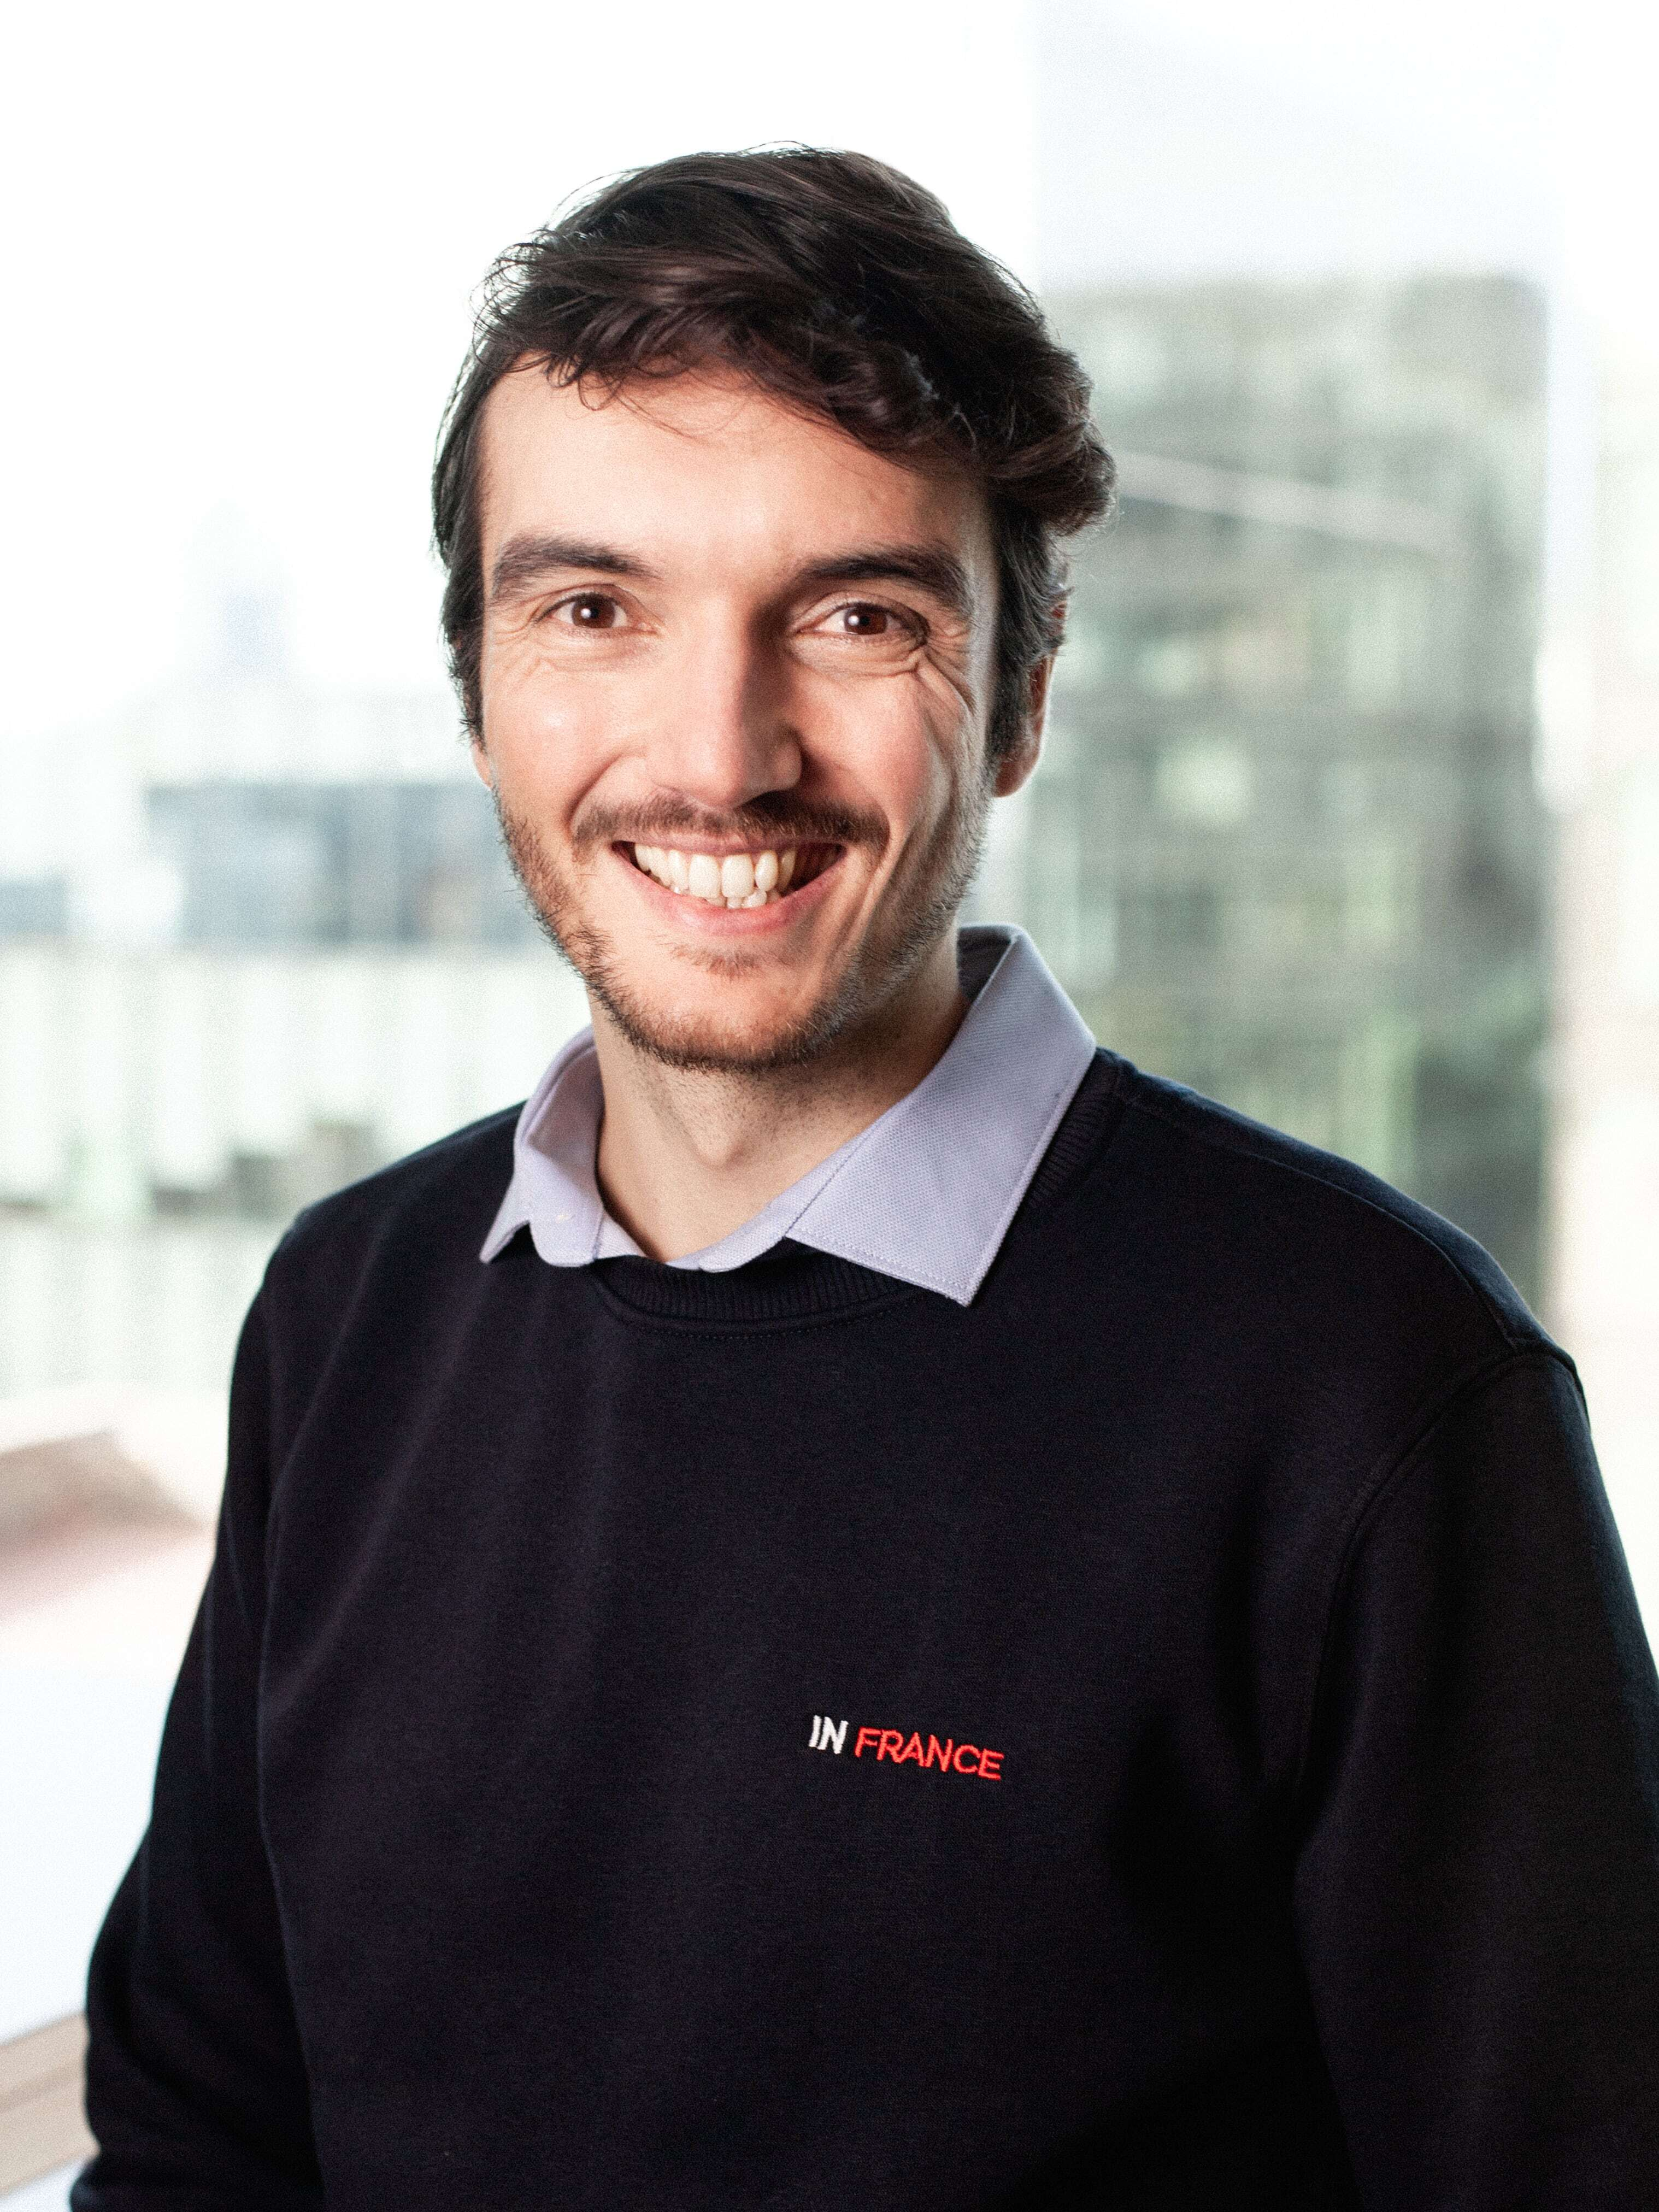
\includegraphics[width=5cm]{image/trombine-christophe.jpg}
        \end{columns}
    \end{frame}


    \section{Généralités}

    \begin{frame}
        \transdissolve
        \frametitle{Les ressources matérielles}
        \framesubtitle{Christophe Brun, conseil en développement informatique}
    \end{frame}


    \section{Les différentes architectures d’une application}

\end{document}
